\documentclass[a4paper,12pt]{article}
\usepackage{graphicx}
\usepackage{subcaption}
\usepackage[bottom]{footmisc}
\begin{document}

\setlength{\parindent}{0pt}
\setlength{\parskip}{6pt}


\title{My First Document}\author{My Name}\date{\today}\maketitle

\pagenumbering{roman}\tableofcontents\newpage\pagenumbering{arabic}

\section{Results}
\subsection{Output}
\subsubsection{Typical simluations}

A simulation = .... show picture : genes, field, network
=> show two picture, one with also model SS2
Genes = weighted over 8 bits : values between $0$ and $2^8 - 1$

this should be much longer


so as figures don't run into one another... 

otherwise learn to skip pages...

Mostly will be working with average for relative value for genes over the pop / after a lot of time
One experiment => results for four genes
Typically (unless specified overwise), values averaged over 30 experiments

\subsubsection{Remembered Heroes}
\label{ss:RH}
These output values are precise to the percentage point. 
For $\bf{SelfSacrifice}$ this poses a problem, as final values are expected to be relatively
small - with typical parameter values (as in \textbf{section 2}), average probability of self-sacrifice
 is capped at 2-3\%.

For this reason, simulations also kept track of $\bf{RememberedHeroes}$, a measure for the number of heroes 
in the live memory of a society. At each simulation step (year), the number of "voluntary" martyrs was computed
 by subtracting the expected number of martyrs which could be solely attributable to mutations in a population
 that did not engage in self-sacrifice. These were added to the number of heroes which could be assumed to have
 been \emph{witnessed} by (alive) individuals in the population. In a given year, $\bf{RememberedHeroes}$ corresponds
 to the number of heroes witnessed by at least \emph{RemThreshold} percent of the population (5 \% in practice).
 In situations where self-sacrificial behavior can be said to be absent, $\bf{RememberedHeroes}$ is close to 0
 (e.g. when \emph{Admiration} is null in the first model under).

\subsection{Exogenous model: simulation outputs}

\subsubsection{Main results}

\begin{figure}[h]
\centering
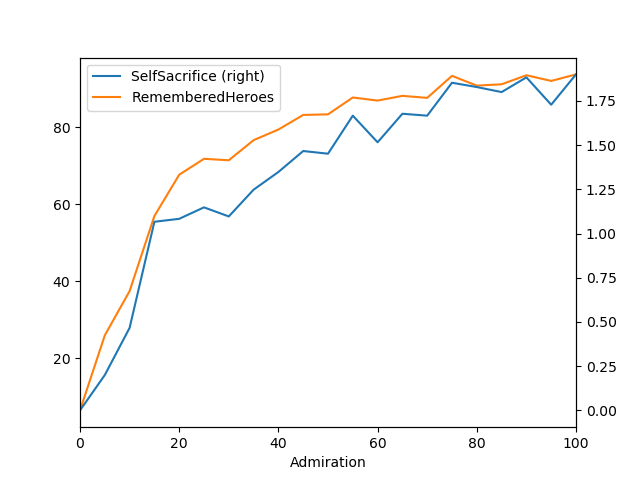
\includegraphics[width=1\textwidth]{RGT_10}
\caption{$\bf{SelfSacrifice}$ and $\bf{RememberedHeroes}$, as a function of \emph{Admiration} (typical parameter values).}
\label{fig:RGT_10}
\end{figure}



\textbf{Figure \ref{fig:RGT_10}} shows results obtained by averaging over 30 simulations, according to the \emph{Admiration}
 parameter (all others being kept constant at the previously described values). As could be expected, $\bf{RememberedHeroes}$
 rises from 0 with \emph{Admiration}, quickly reaching two thirds of its maximum value of under 100 heroes when
 \emph{Admiration} exceeds 20. 
 
 $\bf{SelfSacrifice}$ follows similar dynamics, with values ranging between 0 and 2\% (values to a higher precision than
 the percentage point being obtained artificially by averaging over experimental results). These values are far from negligible:
 for a typical population of 200, we expect an average of (almost) 4 martyrs each year.
 Such collective behavior is captured here by individuals all bearing similar genetic probability $P$
 of self-sacrifice at equilibrium (and obtaining similar $\bf{Reproductive\_points}$ in the 
 long-term), as seen on \textbf{Figure \ref{fig:Snap}}. 
 
 \begin{figure}[h]
    \centering
    \begin{subfigure}[b]{0.3\linewidth} 
        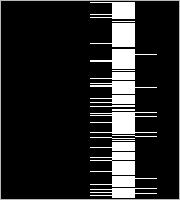
\includegraphics[width=\linewidth, height =\linewidth]{Exo_Genome}
        \caption{Genetic values}
    \end{subfigure}
    \begin{subfigure}[b]{0.3\linewidth}
        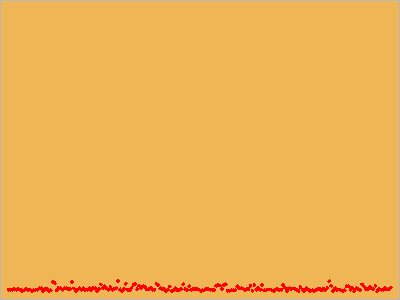
\includegraphics[width=\linewidth, height = \linewidth]{Exo_Field}
        \caption{Reproductive points}
    \end{subfigure}
    \caption{Snapshot of individual values, \emph{A=50}. An individual's genome is represented by a horizontal line on the left: here most bear a $\bf{SelfSacrifice}$ gene
    of relative value $\frac{2^2}{2^8-1}$ (around $1.6\%$). Individuals (horizontal axis) and their reproductive points (vertical) are represented on the right.}
    \label{fig:Snap}
    \end{figure}


 However, one can also imagine the collectively equivalent situation where only a small fraction $f$ of individuals
 engage in self-sacrificial behavior with higher probability $p$ (with $P = f*p$), to the much more
 significant benefit of their families (see \textbf{Section \ref{sec_exo_math}}).

\subsubsection{Influence of \emph{ReproGainsThreshold} $RGT$}

\begin{figure}[h]
    \centering
    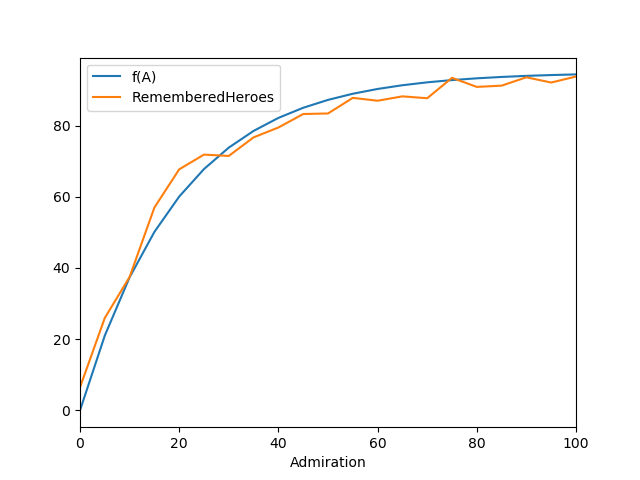
\includegraphics[width=0.6\textwidth]{f_rgt10}
    \caption{$\bf{RememberedHeroes}$ and corresponding optimal $f$ as functions of 
    \emph{Admiration}, for $RGT=10$ ($C=95, \tau = 20$).}
    \label{fig:f_10}
    \end{figure}

As a function of \emph{Admiration}, $\bf{RememberedHeroes}$ resembles a function of the form:
$f_{C,\tau}(t) = C*(1-exp(-t/\tau))$.
% Com sur la forme de la fonction ? Par ex: selection d'une allele, cf Nettle p80
% ou radioactive decay / pop growth with ...
Very approximately\footnote{By choosing optimal C and $\tau$ at a precision of 5 units;
the idea here being simply to get a "feel" for overall variation with $A$. Optimal parameters are the
ones for which Euclidean distance is minimal.},
it can best be approached by a function of this form with parameters $C=95$ and $\tau = 20$, as visible
on \textbf{Figure \ref{fig:f_10}}.

\begin{figure}[h]
    \centering
    \begin{subfigure}[b]{0.4\linewidth} 
        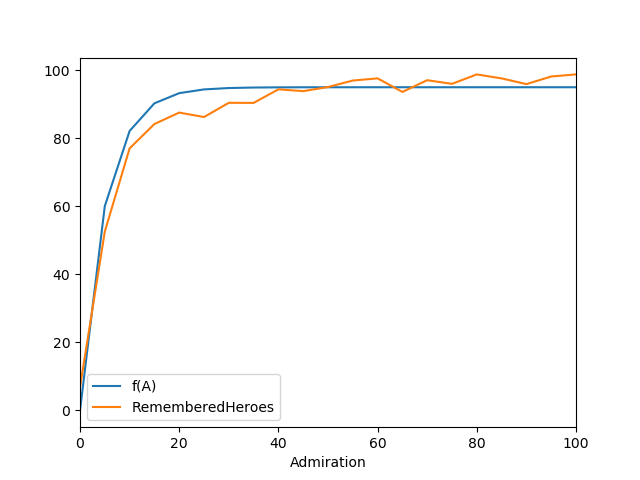
\includegraphics[width=\linewidth]{f_rgt5}
        \caption{$RGT=5$ ($C=95,\tau=5$)}
    \end{subfigure}
    \begin{subfigure}[b]{0.4\linewidth}
        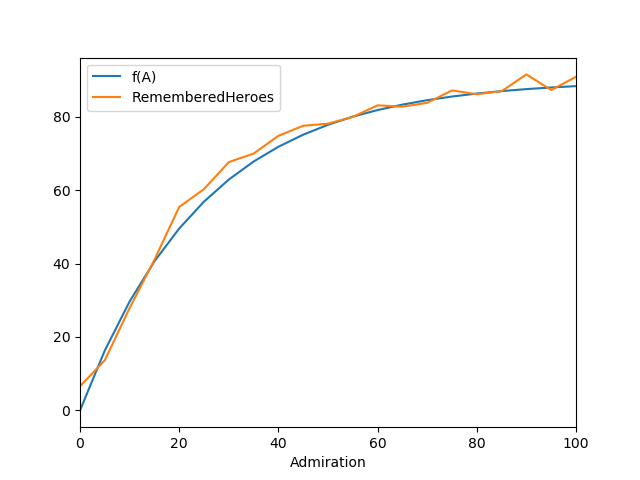
\includegraphics[width=\linewidth]{f_rgt20}
        \caption{$RGT=20$ ($C=90,\tau=25$)}
    \end{subfigure}
    \caption{$\bf{RememberedHeroes}$ and $f$ for $RGT=5, 20$}
    \label{fig:RGT5-20}
    \end{figure}

The key parameter governing relative growth of $\bf{RememberedHeroes}$\footnote{
This output's absolute value is arbitrary, chosen according to \emph{RemThreshold} in
order to provide for visible variations (see \textbf{Section \ref{ss:RH}}).
} thus appears to be one equal to two times
\emph{ReproGainsThreshold}. The importance of $RGT$ is not surprising since it plays
the crucial role of defining the unit in which $\bf{Reproductive\_points}$ are counted.  
The relationship between $RGT$ and final results is however non-trivial, since 
variation according to $A$ for $RGT=5$ (resp. $RGT=20$) are best captured by $\tau=5$
(resp. $\tau=25$), as visible on \textbf{Figure \ref{fig:RGT5-20}}; suggesting perhaps
a quadratic relationship between $RGT$ and $\tau$. \textbf{Section \ref{ss: exo_existence}}
returns to this issue.
%%% A MODIF : provides a charac for minimal ESS > 0... et plus si affinites?

\subsubsection{Variation with \emph{SacrificeHeredity} $h$}

%%% Au moins le graphe A = 50 vs h... => et donc ?
Contrary to what could be expected, h -> 1 is a problem: probs because pop = too small
and all end up with same h... - as shown by simu // because same family ? (or just expected in LT?)
h = 0 discontinuity = expected

\subsubsection{Variation with \emph{ReproductionRate} $r$}
%%% Duh, with N... // and also relationship p and r visibly => cf section 1.3.3.

\subsection{Exogenous model: mathematical proof of concept}
\label{sec_exo_math}
%%% BONUS : here add f << 1 : using equation on A * ... / f < RGT...

\subsubsection{Simplifying assumptions and characterization of equilibrium}
\label{ss:exm_eq}
Individuals live to a maximum of \emph{AgeMax} $M$ years, fixed at 40 here. 
 Expected life span is lower however, as individuals face random accidents
 (in a wide sense) and is equal to $\alpha*M$, where $\alpha$ captures
 the effects of natural selection. In this model, all individuals face the same $\alpha$, but
 may obtain differing reproductive opportunities ($\bf{Selectivity}$ mode).

An individual who engages in self-sacrificial behavior with probability $p$
 shortens his/her lifespan by a multiplicative factor of (see \textbf{Appedix \ref{beta}}):
 
\begin{equation}
 \beta(p) = \frac{(1-p) - (1-p)^{(M+1)}}{p*M} 
\label{eq_beta}
\end{equation}

As such, said individual's reproductive window is shorter, which should lead to the disappearance of
 self-sacrificial behavior - unless this is compensated by increased reproductive opportunities. In contrast to how the
 actual simulation is played, let us assume that: 
 \begin{itemize}
\item Only a \textit{negligible proportion $f$} of individuals engage in self-sacrificial behavior, with equal probability $p$;
\item These future "heroes" will be the first this society sees (everyone starts off with no $\bf{Reproductive\_points}$ $RP$);
\item Generations do not overlap;
\item Individuals are granted their lifetime reproductive potential $R$ at birth
(in contrast with a year-by-year attribution).
\end{itemize}
 
In such a situation, individuals who engage in self-sacrificial behavior obtain on average $\alpha*\beta(p)*M*r$ offspring, 
with others obtaining $\alpha*M*r$, where $r$ is the population-level \emph{ReproductionRate}. However,
the former's children are granted a larger reproduction potential $R_+(A,f)$, which notably
depends on \emph{Admiration} $A$. Since $f$ is assumed to be very small, $R_+(A,f)$ is the same for all
children of individuals who self-sacrifice (we neglect the possibility of individuals being born from two
would-be martyrs), and the children of non-would-be martyrs obtain a reproductive potential which can be
approximated to $r$.

If, in addition, we assume that \emph{$p$ and $M$ are sufficiently large}\footnote{We still expect
$P=f*p$ to be relatively small, to avoid "martyr over-crowding",
but for this to be primarily due to $f$, in the current mathematical characterization.}
for would-be heroes to largely end up
actually laying their life for the group (and not dying in another way), such individuals obtain 
on average $R_+(A,f)*\alpha*\beta(p)*M*r$ grand-children, while others obtain $\alpha*M*r^2$. Thus, a first-order
(neglecting the effects on subsequent generations) characterization of equivalence between both strategies can be written as:
%p and M large debatable ?? Not that much, maybe add a note /// add that we still expect P to be small
 
\begin{equation}
    R_+(A,f)*\beta(p) = r
\label{eq:grandchildren}
\end{equation}
%% le environ egal devient egal...

%%%% POURQUOI JLD VOULAIT RAJOUTER DES f???

\subsubsection{Existence of a self-sacrifice ESS}
\label{ss: exo_existence}

Let $N$ be equal to \emph{PopulationSize}, implicitly assumed to be large here (since $f$
is negligible). Following the simplifying assumptions made above, total social admiration is
borne from each non-hero in the first generation and is thus equal to $A*N*(1-P)$. For children
of martyrs, two cases are possible:

\begin{itemize}
\item either $\frac{AN(1-P)}{fN*\alpha\beta(p)Mr} < RGT$, and each receives reproductive potential $r$;
\item or $\frac{AN(1-P)}{fN*\alpha\beta(p)Mr} \geq RGT$, and each receives $R_{+}(A,f)>r$.
\end{itemize}


In a population composed of $N-1$ non-heroes and one mutant would-be martyr, the latter will
thus be able to invade if, in particular\footnote{ $\alpha$ and $\beta(p)$ are smaller than 1.}:

\begin{equation}
    A > A_{min} = \frac{RGT*M*r}{N} 
\label{eq:ESS}
\end{equation}


When this condition is met, complete absence of self-sacrifice cannot be an ESS.  

thus, since 
%ca existe tjs un ESS ? Pas sur, c'est plutot l'eq de Nash en strat mixte...


% AN : en fait beta bijection vu le truc...
% on obtient p = 9,3% avec nos valeurs... (which is not too small) /// [and P = p/200 = 0.004] ///
%OK really smally f if you take N big...

% ici mettre la figure pour Beta en fait... ?




%%% BONUS : here add f << 1 : using equation on A * ... / f < RGT...
%\subsubsection{A posteriori justification of $f<<1$}
% ca marche ca ???
%% si condition sur f => condition sur P avec le p d'en-dessous

\subsubsection{Mathematical characterization of the ESS}

%%% COMMENCER ICI / dans l'annexe correspondante : calcul de p a l'eq... (sachant f petit...)
%% => pb pour l'AN ???


As shown in \textbf{Appendix \ref{ss:R+}}, a first-order approximation of $R_+$\footnote{Note that 
all equalities in this section are approximations.} in the latter case is ($S$ is equal to \emph{Selectivity}):
\begin{equation}
    R_+(A,f) = \frac{S*r}{log(1+S)} * (1 - \frac{f*\beta(p)}{2})
\label{eq:R+}
\end{equation}

When \emph{Admiration} is sufficient large, self-sacrifice with overall probability $P=f*p$ is thus an ESS
when $p$ and $f$ verify:

%% le environ egal devient egal...


% bon en vrai y a pas de r, mais on voit l'idee.... RGT gouverne bien le truc : cf les graphes...
% this = really extreme, but then again N*r is not that big...

%% PB : comment ramener le f ???


%MATH + => demo that small proba + ... + ...

















\subsection{"Endogenous" model}
%/actual model...


\section{Perspectives}
\subsection{Limitations}
%Oops NonPatriots that actually self-sacrifice....
\appendix

\section{Python stuff}

\section{Mathematical demonstrations}

\subsection{Exogenous model}
\subsubsection{RemTH}
\subsubsection{$\beta(p)$}
\label{beta}

Disregarding the effects of natural selection (which are the same for all individuals here),
 an individual who bears a $\bf{SelfSacrifice}$ gene of relative value $p$, has a probability $p$ of dying in his first year
 (before being able to foster any descendants), a probability $(1-p)*p$ of dying at age $1$ ...
 a probability $(1-p)^{n}*p$ of dying at age $n<M$ ... and is certain to die at age $M$, should
 he or she reach it. His/her expected life span is thus:

 \[ ELS = p*0 + (1-p)*p*1 + ... + (1-p)^{M-1}*(M-1) + (1-p)^M*M \]

Let $f \colon \mathbf{R} \to \mathbf{R}$ be the polynomial function defined by the expression:
\[ f(x) = \sum_{n=0}^{M-1} p*(1-p)^n*x^n + (1-p)^M*x^M \]

By deriving $f$, one can note that:
\begin{equation}
    ELS = f'(1)
\label{eq_ELS_f}
\end{equation}

$f(x)$ involves a geometric sum and can be simplified to (when $(1-p)*x$ is different than 1):

\[ f(x) = p* \frac{1 - ((1-p)*x)^M}{1-(1-p)*x} + ((1-p)*x)^M \]

For $x\neq\frac{1}{(1-p)}$ ($p=1$ trivially yields $ELS=0$):

\[ f'(x) = p * \frac{-M(1-p)^Mx^{M-1}*(1-(1-p)x) + (1-p)*(1-((1-p)x)^M)}{(1-(1-p)x)^2} + M(1-p)^Mx^{M-1} \]

And thus:

\[f'(1) = p * \frac{(-M(1-p)^M*p + (1-p)*(1-(1-p)^M)}{p^2} + M(1-p)^M \]

\begin{equation}
    f'(1) = \frac{(1-p)*(1-(1-p)^M)}{p}
\label{eq_f'}
\end{equation}

Combining these two expressions for $f'(1)$ proves equation ($\bf\ref{eq_beta}$). \textbf{Figure \ref{fig:beta}} shows
$\beta(p)$ for $p$ between 0 and 1. Factoring in natural selection, an individual's expected life span is therefore equal to: $\alpha*\beta(p)*M$.

\begin{figure}[h]
    \centering
    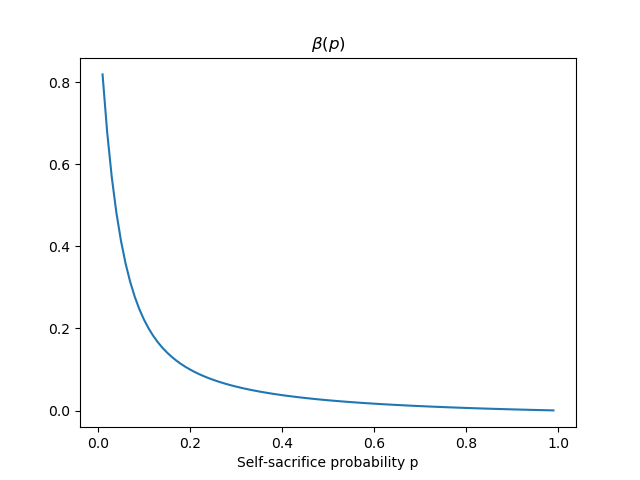
\includegraphics[width=1\textwidth]{Beta}
    \caption{Loss of expected life-span due to self-sacrifice.}
    \label{fig:beta}
    \end{figure}
    



\subsubsection{$R_{+}(A)$}
\label{ss:R+}
In $\bf{Selectivity}$ mode, individuals obtain reproductive potential $R$ according to their
$\bf{Reproductive\_points}$ $RP$, each individual obtains a rank $k$
according to $RP$, and receives reproductive potential:
\[ R = \frac{r}{2} * (\frac{S}
{(S*k + N')*log(1+S)} + \frac{S}{(S*(k+1) + N')*log(1+S)}*N') \]

where $N'<N$ is the number of eligible parents (non-martyrs) and $S$ is equal to \emph{Selectivity}
(the average reproductive potential over eligible parents being \emph{ReproductionRate} $r$).
When $N >> 1$, $R$ verifies:

\begin{equation}
    R \in [R_{min};R_{max}], \textrm{with } R_{max} \approx \frac{S*r}{log(1+S)} 
    \textrm{ and } R_{min} \approx
    \frac{R_{max}}{1+S}
\label{eq:ReproPot}
\end{equation}

With typical parameters ($S=10$ and $r=15\%$), we obtain: $R_{max} \approx 63 \%$ and 
$R_{min} \approx R_{min} \approx 5,6 \%$.

In a case where a negligible proportion $f$ of individuals engage in
self-sacrificial behavior (which is assured to end up in their martyrdom), their children each
receive, on average:
\begin{itemize}
\item reproductive potential $r$, when $\frac{AN(1-P)}{fN*\alpha\beta(p)Mr} < RGT$;
\item $R_{+}(A,f)$ otherwise, as seen in \textbf{Section \ref{ss: exo_existence}}.
\end{itemize}

When $N>>1$, expected $R_+(A,f)$ is equal to the average between the "luckiest" ($k=0$) and "unluckiest"
child, which is approximately:
\[ R_+(A,f) \approx \frac{S*r}{2*log(1+S)} * (1 + \frac{N'}{S*fN*\alpha\beta(p)Mr+N'})\]

\[ R_+(A,f) \approx \frac{S*r}{2*log(1+S)} * (1 + \frac{1}{\frac{S*fN*\alpha\beta(p)Mr}{(1-f)N*\alpha Mr + fN*\alpha\beta(p)Mr}+1})\]

\[ R_+(A,f) \approx \frac{S*r}{2*log(1+S)} * (1 + \frac{(1-f) + f\beta(p)}{(S+1)*f*\beta(p)+(1-f)})\]

Which yields, for $f<<1$ (neglecting terms of order 2 and above):

\begin{equation}
    R_+(A,f) \approx  \frac{S*r}{log(1+S)} * (1 - \frac{f*\beta(p)}{2}) = R_{max}*(1-\frac{f\beta(p)}{2})
\label{eq:R+}
\end{equation}


\end{document}


%Tous les calculs sont faits en moyenne / esperance... pas precise a chaque fois ?